% This line is intentionally within the first four lines for arXiv compatibility.
\pdfoutput=1
\documentclass[aps,prd,amsmath,floats,floatfix,onecolumn,compact,superscriptaddress,nofootinbib]{revtex4-2}

% Encoding and fonts
\usepackage[T1]{fontenc}
\usepackage[utf8]{inputenc}
\usepackage{lmodern}

% Math and symbols
\usepackage{amsmath}
\usepackage{amssymb}
\IfFileExists{bm.sty}{\usepackage{bm}}{}
\IfFileExists{tensor.sty}{\usepackage{tensor}}{}

% Figures and floats
\usepackage{graphicx}
\usepackage{tikz}
\usetikzlibrary{positioning,arrows.meta}

% Colors and hyperlinks
\usepackage[dvipsnames,usenames]{xcolor}
\definecolor{linkcolor}{rgb}{0.0,0.3,0.5}
\definecolor{darkblue}{rgb}{0.0,0.0,0.55}
\usepackage[hypertexnames=false,unicode,colorlinks=true,linkcolor=linkcolor,citecolor=linkcolor,filecolor=linkcolor,urlcolor=linkcolor,pdfusetitle]{hyperref}

% Writing utilities
\usepackage{xspace}
\usepackage[english]{babel}

\graphicspath{{figures/}}

% Compact one-column layout controls.
\setlength{\parskip}{0pt}
\setlength{\textfloatsep}{8pt plus 2pt minus 2pt}
\setlength{\floatsep}{8pt plus 2pt minus 2pt}
\setlength{\intextsep}{8pt plus 2pt minus 2pt}
\setlength{\abovedisplayskip}{6pt plus 2pt minus 2pt}
\setlength{\belowdisplayskip}{6pt plus 2pt minus 2pt}
\renewcommand{\baselinestretch}{0.98}
\allowdisplaybreaks

% Shared macros for the manuscript.
% Keep paper-wide macros here rather than in section files.

\newcommand{\TODO}[1]{\textcolor{red}{\textbf{TODO: #1}}}
\newcommand{\Note}[1]{\textcolor{blue}{\textbf{[#1]}}}
\newcommand{\etal}{\textit{et al.}\xspace}
\newcommand{\ie}{i.e.\xspace}
\newcommand{\eg}{e.g.\xspace}

% Default figure macro. The required default width is 0.8\columnwidth.
\newcommand{\paperfig}[4][0.8\columnwidth]{%
\begin{figure}[htbp]
    \centering
    \includegraphics[width=#1]{#2}
    \caption{#3}
    \label{#4}
\end{figure}%
}

% Default table skeleton for consistent spacing.
\newcommand{\papertable}[3]{%
\begin{table}[htbp]
    \centering
    \caption{#1}
    \label{#2}
    #3
\end{table}%
}
\newcommand{\hateq}{\mathrel{\hat=}}
\newcommand{\varh}{h_{\rm tr}}


% NEW-FORMULATION highlighting: everything original to Z4c-CCM is dark blue;
% transcribed background equations (Refs. [1-3]) remain black.
\newcommand{\nf}[1]{{\color{darkblue}#1}}
\newenvironment{nfblock}{\par\begingroup\color{darkblue}}{\endgroup\par}

%%%%%%%%%%%%%%%%%%%%%%%%%%%%%%%%%%%%%%%%%%%%%%%%%%%%%%%%%%%%%%%%%%%%%%%%%%%
\begin{document}

\title{Cauchy--characteristic matching for the Z4c evolution system}

\author{z4c-CMM verified research loop}
\affiliation{Generated from the z4c-CCM knowledge ledger
(\texttt{knowledge-database/paper\_z4c-CCM/}); every equation and number
below is traceable to a verifier output under \texttt{results/numerical/}.}

\date{\today}

\begin{abstract}
We formulate Cauchy--characteristic matching (CCM) for the Z4c
formulation of the Einstein equations and verify it as a single closed
derivation chain. The ten incoming characteristic modes of the Z4c outer
boundary are classified and assigned data sources; the two physical
modes carry the incoming Weyl scalar $\psi_0$ from a characteristic
evolution through an exact incoming-Weyl dictionary and a Type-II boost,
while the constraint and gauge modes retain absorbing
constraint-preserving conditions. On the characteristic side we give the
linear $\ell=2$ Bondi--Sachs hierarchy in a $\beta$-corrected, unringed
form that admits worldtube data in the gauge naturally produced by a
live Cauchy state, together with a gauge-invariant $\psi_0$ extraction
whose anchored-gauge tails are exactly silent. A local six-row worldtube
map and a retarded matching geometry close the two-way coupling in
process. The formulation is verified against an exact finite-radius
Teukolsky waveform (measured sixth-order convergence), an independent
production characteristic code on identical worldtube data (agreement to
$6\times10^{-6}$ in the waveform and $0.1\%$ in the datum), and the
published simulation data of the reference CCM study. Every equation is
labeled by its source: a machine-verified result of this program,
standard literature, or an explicitly open obligation.
\end{abstract}

\maketitle

\section{Introduction}
\label{sec:intro}

Cauchy--characteristic matching (CCM) couples a strongly hyperbolic
interior (Cauchy) evolution to a characteristic evolution reaching future
null infinity, so that the worldtube supplying characteristic boundary
data simultaneously receives the incoming radiative content computed on
the characteristic grid; the interface becomes transparent rather than
approximately absorbing \cite{Ma:2023qjn,Moxon:2020gha}. The present
paper formulates and verifies CCM for the Z4c formulation of the Einstein
equations \cite{Bernuzzi:2009ex,Hilditch:2012fp,Ruiz:2010qj}: the
constraint-damped conformal decomposition in production use across
finite-difference numerical-relativity codes, here the AthenaK
implementation \cite{Zhu:2024utz}. The presentation follows the
organization of Ref.~\cite{Ma:2023qjn}: the Cauchy system and its
boundary sector (Sec.~\ref{sec:cauchy}), the characteristic system
(Sec.~\ref{sec:characteristic}), the matching algorithm
(Sec.~\ref{sec:matching}), and numerical verification
(Sec.~\ref{sec:tests}). Every equation is one of: (a) a machine-verified
result of this program (dark blue; verification labels [V$n$] and the
ledger nodes N$1$--N$16$); (b) standard literature content, cited at the
equation; (c) an explicitly open obligation (labels O-N$x$-$y$). The
derivation chain is summarized as a directed acyclic graph in
Fig.~\ref{fig:dag}.

\section{The Z4c Cauchy system and its boundary sector}
\label{sec:cauchy}

Black equations are standard literature content, cited at the equation; \nf{dark blue} equations are the machine-verified new Z4c-CCM content (verification labels [V$n$], Table~\ref{tab:static}; ledger nodes in section titles).
\subsection{Boundary frame and Z4c variables}
\label{sec:frame}

\begin{equation}
ds^2 = -\alpha^2\,dt^2 + \gamma_{ij}\,(dx^i+\beta^i dt)(dx^j+\beta^j dt),
\qquad
n^\mu = \alpha^{-1}\,(1,\,-\beta^i),
\label{eq:adm}
\end{equation}
\begin{equation}
s_i = \frac{\partial_i r}{\sqrt{\gamma^{rr}}},\qquad
s^i = \frac{\gamma^{ir}}{\sqrt{\gamma^{rr}}},\qquad
m^A = \tfrac{1}{\sqrt{2}}\big(e_2 + i\,e_3\big)^A,
\label{eq:normal}
\end{equation}
\begin{equation}
\mathring{l}^\mu = \tfrac{1}{\sqrt{2}}\,(n^\mu + s^\mu),\qquad
\mathring{k}^\mu = \tfrac{1}{\sqrt{2}}\,(n^\mu - s^\mu)
\qquad\text{\cite{Ruiz:2010qj}}.
\label{eq:nullvecs}
\end{equation}
Z4c variables \cite{Ruiz:2010qj}:
\begin{equation}
\chi = (\det\gamma)^{-1/3},\quad
\tilde\gamma_{ij} = \chi\,\gamma_{ij},\quad
K = \hat K + 2\Theta,\quad
\tilde A_{ij} = \chi\Big(K_{ij}-\tfrac{1}{3}\gamma_{ij}K\Big),
\label{eq:z4cvars}
\end{equation}
\begin{align}
\partial_t \chi &= \tfrac{2}{3}\,\chi\,\big[\alpha(\hat K + 2\Theta) - D_i\beta^i\big],
\label{eq:dtchi}\\
\partial_t \tilde\gamma_{ij} &= -2\alpha \tilde A_{ij}
 + \beta^k \tilde\gamma_{ij,k}
 + 2\tilde\gamma_{k(i}\,\beta^k_{,j)}
 - \tfrac{2}{3}\,\tilde\gamma_{ij}\,\beta^k{}_{,k}
\qquad\text{\cite{Ruiz:2010qj}}.
\label{eq:dtgt}
\end{align}


\subsection{The Z4c evolution system}
\label{sec:z4csys}

The Z4c formulation \cite{Bernuzzi:2009ex,Hilditch:2012fp} --- the
conformal, constraint-damped reduction of the covariant Z4 system
\cite{Bona:2003fj} --- evolves the
conformal variables \eqref{eq:z4cvars} together with
$\hat K = K - 2\Theta$, the conformal trace-free curvature
$\tilde A_{ij}$, the constraint pair $(\Theta, Z_i)$ --- with $Z_i$
carried by $\tilde\Gamma^i = \tilde\gamma^{jk}\tilde\Gamma^i_{jk}
 + 2\tilde\gamma^{ij}Z_j$ --- and the gauge $(\alpha,\beta^i)$. In
vacuum, with $D_i$ the $\gamma$-covariant derivative and
$[\cdot]^{\rm TF}$ the $\gamma$-trace-free part, the evolution equations
are \cite{Bernuzzi:2009ex}
\begin{align}
\partial_t \hat K &= \beta^i\partial_i\hat K - D^iD_i\alpha
 + \alpha\Big[\tilde A_{ij}\tilde A^{ij}
 + \tfrac13\big(\hat K + 2\Theta\big)^2\Big]
 + \alpha\,\kappa_1\big(1-\kappa_2\big)\,\Theta,
\label{eq:dtKhat}\\
\partial_t \tilde A_{ij} &= \beta^k\partial_k\tilde A_{ij}
 + 2\tilde A_{k(i}\partial_{j)}\beta^k
 - \tfrac23\,\tilde A_{ij}\,\partial_k\beta^k
 + \chi\big[\alpha\,R_{ij} - D_iD_j\alpha\big]^{\rm TF}
 + \alpha\Big[\big(\hat K + 2\Theta\big)\tilde A_{ij}
 - 2\,\tilde A_{ik}\tilde A^k{}_j\Big],
\label{eq:dtAt}\\
\partial_t \Theta &= \beta^i\partial_i\Theta
 + \tfrac{\alpha}{2}\Big[\mathcal R + \tfrac23\big(\hat K+2\Theta\big)^2
 - \tilde A_{ij}\tilde A^{ij}\Big]
 - \alpha\,\kappa_1\big(2+\kappa_2\big)\,\Theta,
\label{eq:dtTheta}\\
\partial_t \tilde\Gamma^i &= \beta^k\partial_k\tilde\Gamma^i
 - \tilde\Gamma^k\partial_k\beta^i
 + \tfrac23\,\tilde\Gamma^i\partial_k\beta^k
 + \tilde\gamma^{jk}\partial_j\partial_k\beta^i
 + \tfrac13\,\tilde\gamma^{ij}\partial_j\partial_k\beta^k
 \nonumber\\&\quad
 - 2\,\tilde A^{ij}\partial_j\alpha
 + 2\alpha\Big[\tilde\Gamma^i{}_{jk}\tilde A^{jk}
 - \tfrac32\,\tilde A^{ij}\partial_j\ln\chi
 - \tfrac13\,\tilde\gamma^{ij}\partial_j\big(2\hat K+\Theta\big)
 - \kappa_1\,\tilde\gamma^{ij}Z_j\Big],
\label{eq:dtGam}
\end{align}
with $\mathcal R$ the Ricci scalar of $\gamma_{ij}$ and
$(\kappa_1,\kappa_2)$ the constraint-damping parameters (production:
$\kappa_1 = 0.02$, $\kappa_2 = 0$). The gauge is 1+log slicing and the
gamma-driver shift \cite{Bernuzzi:2009ex,Zhu:2024utz},
\begin{equation}
\partial_t\alpha = \beta^i\partial_i\alpha
 - \mu_L\,\alpha^2\,\hat K,
\qquad
\partial_t\beta^i = \mu_S\,\tilde\Gamma^i - \eta\,\beta^i
 + \beta^j\partial_j\beta^i,
\label{eq:gauge}
\end{equation}
(AthenaK realization: $\mu_L = 2/\alpha$, $\mu_S = 1$, $\eta = 2$
\cite{Zhu:2024utz}). The constraints are
\begin{equation}
\mathcal H = \mathcal R + \tfrac23 K^2 - \tilde A_{ij}\tilde A^{ij},
\qquad
\mathcal M_i = D^j\big(K_{ij} - \gamma_{ij}K\big),
\qquad
\Theta = 0,\qquad Z_i = 0,
\label{eq:constraints}
\end{equation}
and at the principal level the constraint subsystem propagates as waves,
$\Box\Theta \simeq 0 \simeq \Box Z_i$ \cite{Ruiz:2010qj}, the fact
underlying the boundary rows of Sec.~\ref{sec:bcrows} and the stability
analysis of node N13.


\subsection{The ten incoming boundary modes}
\label{sec:modes}

At a timelike outer boundary with frame
\eqref{eq:adm}--\eqref{eq:nullvecs}, the linearized Z4c system carries
ten incoming characteristic fields (taxonomy verified at nodes N4/N5:
transverse-traceless = physical; $h_{ss}$ = gauge; $h_{sA}$ =
constraint-vector; tangential trace = constraint-scalar):
\begin{table}[htbp]
\centering
\caption{Incoming boundary modes of Z4c-CCM and their data sources
(ledger node N6). Per-speed outgoing characteristic vectors
$\mathring X^a = (\mathring n^a + \sqrt{v}\,\mathring s^a)/\sqrt2$ at
sector speed $v$ \cite{Ruiz:2010qj}; production order $L \ge 1$.}
\label{tab:modes}
\footnotesize
\begin{tabular}{cllll}
\hline\hline
\# & sector & incoming field & speed & boundary condition (datum) \\
\hline
1--2 & physical & $U^-_{AB} = {\rm TT}_2[E+\epsilon(s)B]_{AB}$ & $1$ &
 $U^-_{AB} \hateq -(\psi_0'\,\bar m_A\bar m_B + {\rm c.c.})$
 \;[CCM: $\psi_0' = A^2\psi_0^{\rm CCE}$] \\
3 & constraint & $\Theta$ & $1$ &
 $(r^2\,\mathring l\cdot\partial)^{L+1}\,\Theta \hateq 0$ \\
4 & constraint & $Z_s$ & $1$ &
 $(r^2\,\mathring l\cdot\partial)^{L+1}\,Z_s \hateq 0$ \\
5--6 & constraint & $Z_A$ & $1$ &
 $(r^2\,\mathring l\cdot\partial)^{L+1}\,Z_A \hateq 0$ \\
7 & gauge & $\alpha$ & $\sqrt{\mu_L}$ &
 $(r^2\,\mathring m\cdot\partial)^{L+1}\,\alpha \hateq h_\alpha$ \\
8 & gauge & $\beta_s$ & $\sqrt{\nu_s}$ &
 $(r^2\,\mathring k_{\nu_s}\!\cdot\partial)^{L+1}\,\beta_s \hateq h_s$ \\
9--10 & gauge & $\beta_A$ & $\sqrt{\mu_S}$ &
 $(r^2\,\mathring j\cdot\partial)^{L+1}\,\beta_A \hateq h_A$ \\
\hline\hline
\end{tabular}
\end{table}
The constraint and gauge rows are those of Ref.~\cite{Ruiz:2010qj}
adapted to the Z4c variable set; the physical rows 1--2 carry the CCM
datum and constitute the new content (Secs.~\ref{sec:n2}--\ref{sec:n3},
\ref{sec:bcrows}). With $\psi_0'\to0$ the set reduces exactly to the
absorbing constraint-preserving scheme of Ref.~\cite{Ruiz:2010qj} [V6].
The frozen-coefficient LF/GKS analysis of the constraint rows (node N13)
shows that every matched-falloff advection realization of rows 3--6 is
stable and absorbs the $(\Theta,Z_s)$ pair at
$1-O\big((\sigma/2\omega r)^2\big)$, that falloff-mismatched sink
variants self-generate $O(10\%)$ pair reflection, and that the production
default (the stock matched realization) is the admissible optimum.

\subsection{Tetrad correspondence and Type-II boost (node N2)}
\label{sec:n2}

Outgoing null label $u$ with $u|_{\partial\Omega}=t$:
$\partial_\mu u = (1,\,u_r,\,0,\,0)$,
\begin{equation}
g^{tt} + 2g^{tr}u_r + g^{rr}u_r^2 = 0
\quad\Longrightarrow\quad
u_r = \frac{-g^{tr}-\sqrt{(g^{tr})^2 - g^{tt}g^{rr}}}{g^{rr}},
\qquad u_r\big|_{\rm flat} = -1 .
\label{eq:uroot}
\end{equation}
Characteristic outgoing null vector \cite{Moxon:2020gha,Ma:2023qjn}:
\begin{equation}
\hat l^{\,\mu} = -e^{2\hat\beta}\,g^{\mu\nu}\partial_\nu u .
\label{eq:lhat}
\end{equation}
\begin{nfblock}
For arbitrary $(\alpha,\beta^i,\gamma_{ij})$,
\begin{equation}
\mathring{l}^{\mu}
 = \frac{\sqrt{2}}{2}\,
 \big(\alpha-\gamma_{ij}\beta^i s^j\big)\,e^{-2\hat\beta}\;
 \hat l^{\,\mu}
\qquad\text{[V1: exact at 12 rational points; GPU residual
$9.3\times10^{-16}$]},
\label{eq:boost-identity}
\end{equation}
\begin{equation}
A = \big(\alpha-\gamma_{ij}\beta^i s^j\big)\,e^{-2\hat\beta},
\qquad
\psi_0' = A^2\,\psi_0 ,
\label{eq:boost}
\end{equation}
i.e.\ the Choice-2 boost of Ref.~\cite{Ma:2023qjn} holds verbatim on the Z4c
frame \eqref{eq:nullvecs}: no evolution-system variable enters
\eqref{eq:boost-identity}.
\end{nfblock}
$\psi_0$ on the characteristic grid \cite{Moxon:2020gha,Ma:2023qjn}:
\begin{equation}
\psi_0=\Big(\frac{r\partial_{r}\beta-1}{4Kr}\Big)
\Big[(1{+}K)\partial_{r}J-\frac{J^2\partial_{r}\bar{J}}{1{+}K}\Big]
+\frac{J(1{+}K^2)\,\partial_{r}J\,\partial_{r}\bar{J}}{8K^3}
+\frac{1}{8K}\Big[\frac{J^2\partial^2_{r}\bar{J}}{1{+}K}
 -(1{+}K)\partial_{r}^2J\Big]
-\frac{J\bar{J}^2(\partial_{r}J)^2+J^3(\partial_{r}\bar{J})^2}{16K^3}.
\label{eq:psi0cce}
\end{equation}

\subsection{Physical-mode dictionary (node N3, exact)}
\label{sec:n3}

Electric/magnetic Weyl decomposition w.r.t.\ $n^\mu$ (vacuum):
\begin{equation}
E_{\mu\nu} = C_{\mu\alpha\nu\beta}\,n^\alpha n^\beta,
\qquad
B_{\mu\nu} = \tfrac12\,\epsilon_{\mu\alpha}{}^{\gamma\delta}
             C_{\gamma\delta\nu\beta}\,n^\alpha n^\beta,
\qquad
\epsilon_{\mu\nu\rho\sigma}=\sqrt{-g}\,[\mu\nu\rho\sigma].
\label{eq:ebdef}
\end{equation}
\begin{nfblock}
EXACT identity (pure Weyl algebra, generic 10-component tensor; no
perturbation, no field equations) [V2a]:
\begin{equation}
\big(E_{\mu\nu} + \epsilon_{\mu}{}^{\kappa\lambda}s_\kappa
 B_{\lambda\nu}\big)\,m^\mu m^\nu \;=\; -\,\psi_0,
\qquad
\big(E_{\mu\nu} - \epsilon_{\mu}{}^{\kappa\lambda}s_\kappa
 B_{\lambda\nu}\big)\,m^\mu m^\nu \;=\; -\,\bar\psi_4,
\label{eq:exact-dictionary}
\end{equation}
with $\psi_0 = -C_{abcd}\,l^a m^b l^c m^d$ on the frame \eqref{eq:nullvecs};
dyad completeness ($U_{AB} = U(m,m)\,\bar m_A \bar m_B + \mathrm{c.c.}$ for
tangential trace-free $U$) gives the tensor form of the incoming Weyl object
\begin{equation}
U^-_{AB} \;\equiv\; \mathrm{TT}_2\big[E + \epsilon(s)B\big]_{AB}
 \;=\; -\big(\psi_0\,\bar m_A \bar m_B + \bar\psi_0\, m_A m_B\big).
\label{eq:uminus}
\end{equation}
Realization from the Z4c state (Gauss--Codazzi, on-shell vacuum;
$\gamma_{ij}, K_{ij}$ from \eqref{eq:z4cvars}) [V2c]:
\begin{equation}
E_{ij} = R_{ij}[\gamma] + K\,K_{ij} - K_{ik}K^k{}_j,
\qquad
B_{ij} = \epsilon_i{}^{kl}\,D_k K_{lj}\big|_{\rm sym},
\qquad
\epsilon_{ikl} = \sqrt{\det\gamma}\,[ikl].
\label{eq:gausscodazzi}
\end{equation}
\end{nfblock}
Nonperturbative verification (Kerr--Schild Schwarzschild, autodiff, both
routes; Table~\ref{tab:static} V2c): $|E^{3+1}{-}E^{4D}|$ rel.\
$7.7{\times}10^{-17}$, $|B^{3+1}{-}B^{4D}|$ rel.\ $3.9{\times}10^{-17}$,
identity residual $8.5{\times}10^{-16}$. Linearized on-shell flat limit
(superseded defining form, now a corollary [V2b]): for TT $h_{AB}(t,x_s)$,
$\psi_0 = \tfrac14(\partial_t+\partial_s)^2 h_{mm}$ and
$U^-_{AB}\to -\tfrac14 (\partial_t + \partial_s)^2 \gamma^{\rm TF}_{AB}$,
i.e.\ $(\partial_t+\partial_s)^2\gamma^{\rm TF}_{AB}
 = 4(\psi_0 \bar m_A\bar m_B + \mathrm{c.c.})$.

\subsection{The Z4c-CCM boundary conditions (node N6)}
\label{sec:bcrows}
\label{sec:n6}

Ten incoming modes at the worldtube; $X^{\mathring{}}{}^\mu_v =
(n^\mu + \sqrt{v}\,s^\mu)/\sqrt 2$ at sector speed $v$; $L\ge 1$:
\begin{nfblock}
\begin{align}
\text{physical (2):}\qquad &
U^-_{AB} \;\hat=\;
-\Big(\psi_0'\,\bar m_A\bar m_B + \bar\psi_0'\,m_A m_B\Big),
\qquad \psi_0' = A^2\,\psi_0^{\rm CCE}
\quad\text{(exact, \eqref{eq:uminus}--\eqref{eq:gausscodazzi})},
\label{eq:bc-phys}\\
\text{constraint (4):}\qquad &
\big(r^2\,\mathring l\!\cdot\!\partial\big)^{L+1}\,\Theta \;\hat=\; 0,
\qquad
\big(r^2\,\mathring l\!\cdot\!\partial\big)^{L+1}\,Z_s \;\hat=\; 0,
\qquad
\big(r^2\,\mathring l\!\cdot\!\partial\big)^{L+1}\,Z_A \;\hat=\; 0,
\label{eq:bc-cpbc}\\
\text{gauge (4):}\qquad &
\big(r^2\,\mathring m\!\cdot\!\partial\big)^{L+1}\alpha \;\hat=\; 0,
\qquad
\big(r^2\,\mathring k_{\nu_s}\!\!\cdot\!\partial\big)^{L+1}\beta_s \;\hat=\; 0,
\qquad
\big(r^2\,\mathring j\!\cdot\!\partial\big)^{L+1}\beta_A \;\hat=\; 0 .
\label{eq:bc-gauge}
\end{align}
Bj{\o}rhus form of \eqref{eq:bc-phys} (the correction drives the
incoming Weyl object to its CCM value, the Z4c analog of
Ref.~\cite{Ma:2023qjn}):
\begin{equation}
U^-_{AB} - U^-_{AB}\big|_{\rm BC} \to 0,
\qquad
U^-_{AB}\big|_{\rm BC} = -\Big(\psi_0'\,\bar m_A\bar m_B
 + \bar\psi_0'\,m_A m_B\Big);
\qquad
\psi_0^{\rm CCE}\!\to 0 \;\Longrightarrow\; \text{CPBC scheme of
Ref.~\cite{Ruiz:2010qj}}
\quad\text{[V6]}.
\label{eq:bjorhus}
\end{equation}
\end{nfblock}
Equations \eqref{eq:bc-cpbc}--\eqref{eq:bc-gauge} are the order-$L$
conditions of Ref.~\cite{Ruiz:2010qj}; \eqref{eq:bc-gauge} replaces the
Sommerfeld gauge placeholder of Ref.~\cite{Ma:2023qjn}.

\subsection{Sector orthogonality (nodes N4, N5)}
\label{sec:n45}

For arbitrary TT data $h_{AB}(t,x_s)$ [V4]:
\begin{equation}
\mathcal H = \partial_i\partial_j h_{ij} - \partial^2 h^k{}_k = 0,
\qquad
\mathcal M_i = \partial_j \dot h_{ij} - \partial_i \dot h^j{}_j = 0,
\qquad
\gamma^{ij}\partial_t h_{ij} = 0,
\qquad
\tilde\Gamma^i = -\partial_j \tilde h^{ij} = 0 ;
\label{eq:orthogonality}
\end{equation}
negative controls:
$h_{x_s y}=G(t,x_s)\Rightarrow \mathcal M_y = -\tfrac12\,\partial_{x_s}\dot G \neq 0$;
$h_{yy}=h_{zz}=G \Rightarrow \mathcal H = -2\,\partial_{x_s}^2 G \neq 0$.
\begin{nfblock}
Hence the datum \eqref{eq:bc-phys} sources neither
\eqref{eq:bc-cpbc} nor \eqref{eq:bc-gauge} at linear order: the three
sectors of \eqref{eq:bc-phys}--\eqref{eq:bc-gauge} commute.
\end{nfblock}
On the boundary wave model of Ref.~\cite{Ruiz:2010qj},
$\big[\partial_t^2 - 2\mathring\beta\,\partial_t\partial_x
 - (1-\mathring\beta^2)\partial_x^2\big]u = 0$, plane-wave reflection [V5]:
\begin{equation}
R_{\rm Sommerfeld}
 = -\frac{\mathring\beta\,(1-\mathring\beta)}
        {(1+\mathring\beta)(2-\mathring\beta)} \neq 0,
\qquad
R_{(\partial_t + c_+\partial_x)} = 0
\quad\text{(identically)} .
\label{eq:reflection}
\end{equation}

\subsection{Frozen-coefficient boundary stability (node N7)}
\label{sec:n7}

Laplace--Fourier ansatz $u = \tilde u\,e^{st+\lambda x}$, $\Re s>0$ [V7]:
\begin{equation}
\lambda_+ = \frac{s}{1+\mathring\beta}\;(\text{admissible}),
\qquad
\lambda_- = -\frac{s}{1-\mathring\beta},
\qquad
D_L(s) = \Big(s + (1+\mathring\beta)\,\lambda_+\Big)^{L+1} = (2s)^{L+1},
\qquad
\frac{|D_L(s)|}{|s|^{L+1}} = 2^{L+1} .
\label{eq:kreiss}
\end{equation}
\begin{nfblock}
$D_L$ contains no datum symbol: the injection \eqref{eq:bc-phys} modifies
only the inhomogeneity, so the boundary-stability results of
Ref.~\cite{Ruiz:2010qj} (constraint sector: all $L$; gauge+metric sector:
spherical reduction, asymptotically harmonic shift) transfer verbatim with
$\|u\| \le C\,\|\psi_0'\text{-datum}\|$.
\end{nfblock}


\section{The characteristic system}
\label{sec:characteristic}

% iter-2 target: Bondi-Sachs metric + falloffs; the nonlinear
% hypersurface hierarchy (cited); OUR linear l=2 scalarized chain
% (ringed + unringed + machine-derived beta sources); spectral
% solver; psi0 formula + gauge invariance; pulse ID.
\begin{nfblock}
\subsection{Live Cauchy--characteristic matching inside AthenaK
(nodes N13--N14)}
\label{sec:liveccm}

The $\psi_0^{\rm datum}$ provider of \eqref{eq:teuk-inject} is replaced
by a \emph{native, in-process} characteristic solver evolving in
lockstep with the Cauchy evolution (one process, no file round-trips).
On the compactified radial coordinate $y = 1 - 2r_{\rm wt}/r$
(Chebyshev--Gauss--Lobatto collocation, LU-factorized global solves,
SAT time advance), the solver evolves the \emph{unringed} $\ell{=}2$
$t$-scalars $(J_t,Q_t,U_t,W_t,H_t)$ of the linearized Bondi--Sachs
hierarchy with the $\beta$ sources required by live (worldtube-anchored
gauge) data — machine-derived as exact-rational fits on the anchored
and plain solution families jointly:
\begin{align}
\partial_r(r^2 Q) &= -\,r^2\,\partial_r(\bar\eth J) - 4r\,\eth\beta,
&
\partial_r U &= Q/r^2,
\nonumber\\
\partial_r(r^2 W) &= \tfrac12\bar\eth\bar\eth J + 2r\,\bar\eth U
 + \tfrac{r^2}{2}\partial_r(\bar\eth U) - \tfrac43\,\bar\eth\eth\beta,
&
\partial_r(rH) &= \tfrac12 r\,\partial_r^2 J + \partial_r J
 + \frac{\eth^2\beta}{r} - \frac{\eth Q}{2r} - \eth U,
\label{eq:beta-hierarchy}
\end{align}
with $H=\partial_u J$ and $\beta$ $r$-independent at this order. The
ringed variables ($rJ$, $r^2U$, \dots) diverge at scri on anchored-gauge
data ($k=0,1$ tails); the unringed system \eqref{eq:beta-hierarchy} is
regular on $y\in[-1,1]$ in both gauges, and
$\psi_0^t = -\partial_r J_t/(2r) - \partial_r^2 J_t/4$ is gauge-invariant
(the anchored tails are exactly $\psi_0$-silent). Worldtube data are
sampled live from the Cauchy ADM state on three geodesic spheres
($\ell{=}2$ projections; $\partial_t h = -2K$ at linear order) and mapped
by a six-row local contract to the anchored boundary scalars
$(J,Q,U,W,H,\beta)_{\rm wt}$. Cone labeling is retarded, $u = t - r$:
the boundary datum at Cauchy time $t$ is the $\psi_0$ probe at $r_B$ on
the earlier cone $u = t - r_B$ (causality lag, served from a per-substep
history).

\emph{Verification.} (i) Standalone: anchored end-to-end $\psi_0$ probe
within $8.8\times10^{-5}$ of the exact datum
($7.1\times10^{-6}$ at halved step; truncation-dominated). (ii) Live
analytic-stub battery: mode-(solver) vs.\ mode-(self-datum) waveforms
agree to $4.1\times10^{-9}$ of peak. (iii) For the purely outgoing test
the live datum is conditioning-limited \emph{by physics}
($\psi_0/J\sim10^{-8}$ peeling: fidelity would need
$10^{-11}$-relative tube data); the fidelity demonstration instead uses
the characteristic-pulse-injection test of Ref.~\cite{Ma:2023qjn}
Sec.~V.C (ingoing $\ell{=}2$ pulse on the initial null slice, quiescent
Cauchy data, $\psi_0/J = 7\times10^{-3}$): the live datum matches the
verified solver to $7\times10^{-8}$ of peak in the causally clean
window; the transmitted burst exits the Cauchy domain at
$t_2 = t_1 + 2R$ within $0.12$; a no-datum control shows the entire
response is datum-attributable ($2.9\times10^{-10}$ of peak)
[Fig.~\ref{fig:liveccm}(a,b)]. (iv) Cross-oracle: SpECTRE
\texttt{CharacteristicExtract} (the CCE of Ref.~\cite{Ma:2023qjn}), run
on a Bondi--Sachs worldtube file generated from the exact solution,
reproduces $\Psi_4 = -\sqrt{6\pi/5}\,F^{(6)}$ to $6\times10^{-6}$
relative and the datum normalization
$\Psi_0 = -\tfrac98 F^{(2)}$ ($s^2$ shape) to $0.1\%$
[Fig.~\ref{fig:liveccm}(c)]. (v) Constraint rows: a frozen-coefficient
LF/GKS analysis of the $(\Theta, Z_s)$ boundary realizations shows every
matched-falloff advection closure is stable and already absorbs the
constraint pair at $1-O\big((\sigma/2\omega r)^2\big)$; falloff-mismatched
sink rows self-generate $O(10\%)$ pair reflection — the production
default remains the matched (stock) realization of the
\eqref{eq:bc-cpbc} rows.
\end{nfblock}

\begin{figure}[htbp]
\centering
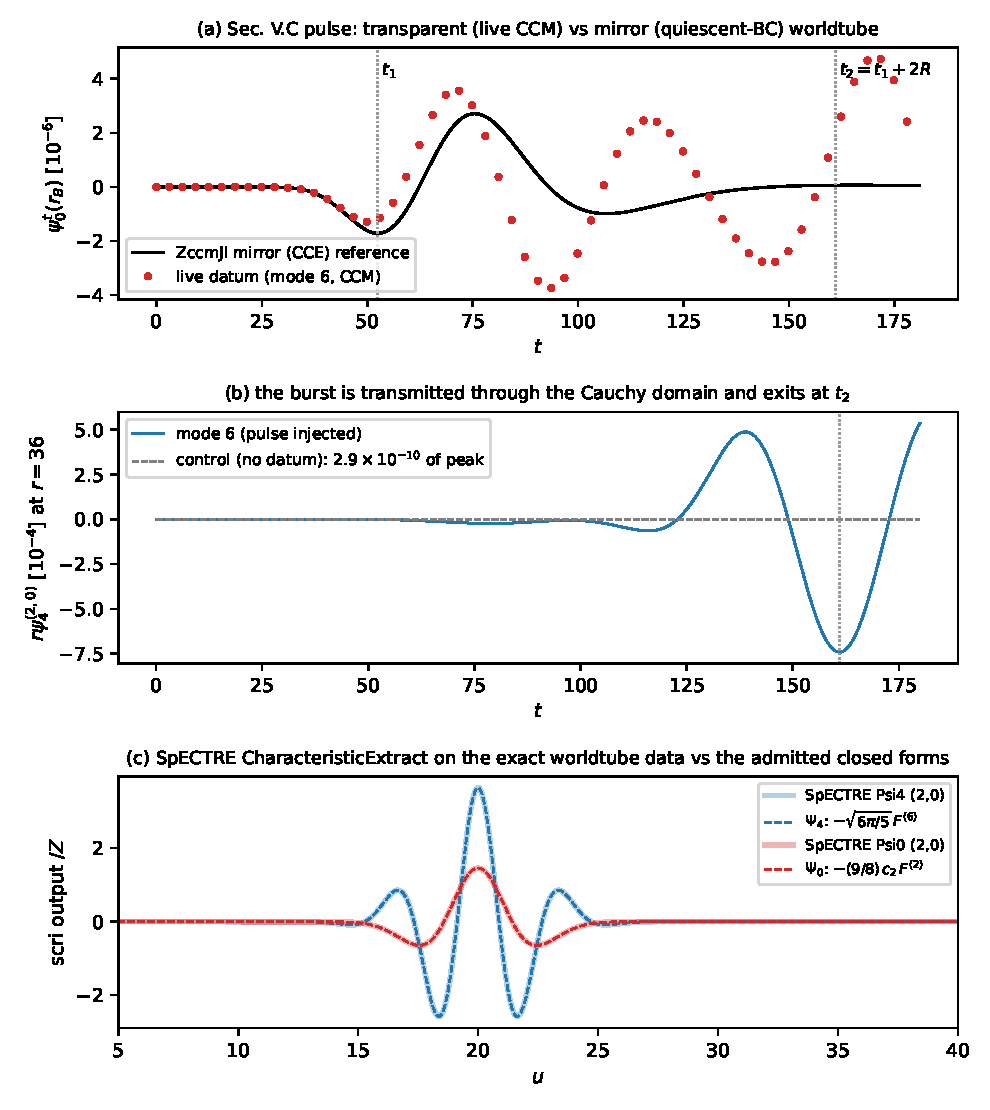
\includegraphics[width=0.8\textwidth]{zccm_live_ccm.pdf}
\caption{Live-CCM results (Sec.~\ref{sec:liveccm}). (a) The
characteristic-pulse fidelity test: live $\psi_0$ datum at the Cauchy
boundary vs.\ the quiescent-worldtube (mirror/CCE) reference — the
early-window agreement is $7\times10^{-8}$ of peak; the later $O(1)$
separation \emph{is} the matching physics (the live run transmits and
later re-receives the pulse). (b) The transmitted burst at the
extraction radius exits at $t_2 = t_1 + 2R$; the no-datum control is
consistent with zero. (c) SpECTRE \texttt{CharacteristicExtract} on the
exact worldtube data vs.\ the closed forms (shaded wide: oracle output;
dashed: $-\sqrt{6\pi/5}F^{(6)}$ and $-\tfrac98 c_2 F^{(2)}$). Generator:
\texttt{scripts/plot\_paper\_figures\_v2.py}; data:
\texttt{results/numerical/n14\_native/}, \texttt{n14\_pulse\_ref.csv},
\texttt{spectre\_oracle/} (ledger nodes N13--N14).}
\label{fig:liveccm}
\end{figure}

\section{The matching algorithm}
\label{sec:matching}

The matching loop closes two data paths each Cauchy step: the worldtube
path (Cauchy state $\to$ characteristic boundary data,
Secs.~\ref{sec:n1}--\ref{sec:wtmap}) and the datum path (characteristic
$\psi_0$ $\to$ the physical boundary rows of Sec.~\ref{sec:bcrows},
Secs.~\ref{sec:retarded}--\ref{sec:cadence}). The full derivation chain
is summarized in Fig.~\ref{fig:dag}.

\subsection{Worldtube data map (node N1)}
\label{sec:n1}

\begin{equation}
g_{00} = -\alpha^2 + \gamma_{ij}\beta^i\beta^j,\qquad
g_{0i} = \gamma_{ij}\beta^j,\qquad
g_{ij} = \gamma_{ij};
\qquad
g^{00} = -\alpha^{-2},\quad
g^{0i} = \frac{\beta^i}{\alpha^{2}},\quad
g^{ij} = \gamma^{ij} - \frac{\beta^i\beta^j}{\alpha^{2}}.
\label{eq:fourmetric}
\end{equation}
ADM kinematics requires
$\partial_t\gamma_{ij} = -2\alpha K_{ij} + \beta^k\partial_k\gamma_{ij}
 + \gamma_{kj}\partial_i\beta^k + \gamma_{ik}\partial_j\beta^k$.
From $\gamma_{ij} = \chi^{-1}\tilde\gamma_{ij}$,
\begin{equation}
\partial_t\gamma_{ij}
 = \chi^{-1}\partial_t\tilde\gamma_{ij}
 - \chi^{-2}\tilde\gamma_{ij}\,\partial_t\chi ,
\label{eq:dtg-step1}
\end{equation}
and inserting \eqref{eq:dtchi}--\eqref{eq:dtgt} with
$K_{ij} = \chi^{-1}\big(\tilde A_{ij}+\tfrac13\tilde\gamma_{ij}K\big)$,
$\beta^k\partial_k\gamma_{ij} = \chi^{-1}\beta^k\partial_k\tilde\gamma_{ij}
 - \gamma_{ij}\,\beta^k\partial_k\ln\chi$,
\begin{equation}
\big[\partial_t\gamma_{ij}\big]_{\rm Z4c}
 - \big[\partial_t\gamma_{ij}\big]_{\rm ADM}
 = \gamma_{ij}\Big[\tfrac{2}{3}\,D_k\beta^k
 - \tfrac{2}{3}\,\partial_k\beta^k
 + \beta^k\partial_k\ln\chi\Big].
\label{eq:dtg-step2}
\end{equation}
\begin{nfblock}
\begin{equation}
\boxed{\;D_i\beta^i = \partial_k\beta^k
 - \tfrac{3}{2}\,\beta^k\,\partial_k\ln\chi\;}
\qquad\text{[V3: closure exact; naive }D=\partial_k\beta^k\text{ leaves
residual }+1\cdot\gamma_{ij}\beta^k\partial_k\ln\chi\text{]}.
\label{eq:divbeta}
\end{equation}
\end{nfblock}

\subsection{Live sampling and the $\ell=2$ data contract}
\label{sec:contract}

\begin{nfblock}
The Cauchy ADM state is interpolated to three geodesic spheres at
$r_{\rm wt}$ and $r_{\rm wt}\pm\delta r$ each step. With orthonormal
frame components $h_{\hat a\hat b} = (\gamma - \delta)_{\hat a\hat b}$
and $\partial_t h_{\hat a\hat b} = -2K_{\hat a\hat b}$ (linear order;
$\alpha = 1 + O(h)$, the correction entering beyond linear), the
$(\ell,m)=(2,0)$ contract scalars are the shape projections
\begin{equation}
h_{\rm TT} = \Big\langle \tfrac12(h_{\hat\theta\hat\theta}
 - h_{\hat\phi\hat\phi})\Big\rangle_{s^2},
\quad
h_{rr} = \big\langle h_{\hat r\hat r}\big\rangle_{P},
\quad
\varh = \big\langle h_{\hat\theta\hat\theta}
 + h_{\hat\phi\hat\phi}\big\rangle_{P},
\quad
h_{r\theta} = \big\langle r\,h_{\hat r\hat\theta}\big\rangle_{sc},
\label{eq:contract}
\end{equation}
with $\langle f\rangle_X = \int f X\,d\Omega / \int X^2\,d\Omega$ for
$X \in \{s^2, P, sc\}$, the time derivatives obtained from the same
projections of $-2K$, and $\partial_r\varh$ by the centered difference
across the sphere triplet. At $\ell=2$ the angular derivatives close
analytically on the same scalars,
\begin{equation}
\big\langle\partial_\theta \varh\big\rangle_{sc} = -6\,\varh,
\qquad
\big\langle\partial_\theta \partial_r\varh\big\rangle_{sc}
 = -6\,\partial_r\varh,
\qquad
\big\langle(\partial_\theta + \cot\theta)\,h_{r\theta}\big\rangle_{P}
 = h_{r\theta},
\label{eq:dthclosures}
\end{equation}
so the contract is seven numbers per step:
$(h_{\rm TT}, \partial_t h_{\rm TT}, h_{rr}, \varh, \partial_r\varh,
 h_{r\theta}, \partial_t h_{r\theta})$.
\end{nfblock}

\subsection{The anchored worldtube map (six rows $+\,\beta$)}
\label{sec:wtmap}

\begin{nfblock}
The Cauchy coordinates near the worldtube do not satisfy the Bondi gauge
conditions; the radial gauge generator is fixed by areal-radius
consistency only up to functions of $(u,\theta)$. Anchoring the
generator to vanish \emph{at the worldtube}, with the angular generator
corrected so that the $g_{r\theta}$ gauge condition holds consistently
($\xi_a = \xi_{\rm old} + \partial_\theta(\zeta_u^{\rm wt})/r -
\text{const}$), makes the map from the contract
\eqref{eq:contract}--\eqref{eq:dthclosures} to the characteristic
boundary scalars \emph{local}:
\begin{align}
J_t^{\rm wt} &= h_{\rm TT},
&
H_t^{\rm wt} &= \partial_t h_{\rm TT},
&
U_t^{\rm wt} &= \frac{6\,\varh}{4\,r_{\rm wt}},
\nonumber\\
Q_t^{\rm wt} &= \frac{6\,\varh}{4} + \frac{6\,r_{\rm wt}\,
\partial_r\varh}{4}
 - \frac{3\,h_{r\theta}}{r_{\rm wt}} + \partial_t h_{r\theta},
&
W_t^{\rm wt} &= \frac{3\,h_{rr}}{4\,r_{\rm wt}}
 - \frac{\partial_r\varh}{4},
&
\beta_t^{\rm wt} &= \frac{h_{rr}}{4} - \frac{\varh}{8}
 - \frac{r_{\rm wt}\,\partial_r\varh}{8}
 + \frac{h_{r\theta}}{4\,r_{\rm wt}},
\label{eq:sixrowmap}
\end{align}
verified as an exact identity against the anchored-gauge solution
series (BigFloat-192 residual $<10^{-35}$; derivation artifact
\texttt{derive\_wtmap\_v2.jl}). The anchored gauge necessarily carries
$\beta_t \neq 0$ and non-decaying tails $a(u) + b(u)/r$ in $J$, $U$,
$W$; these are exactly the structures supported by the
$\beta$-corrected, unringed system \eqref{eq:unringed}, and they are
$\psi_0$-silent by \eqref{eq:psi0formula}. Independent anchoring of the
radial and angular generators violates the $g_{r\theta}$ condition and
is excluded [pinned: the uncorrected map fails the $\beta$ channel with
a characteristic $(4-n)$-ratio pattern].
\end{nfblock}

\subsection{Retarded matching geometry}
\label{sec:retarded}

\begin{nfblock}
The characteristic time is the retarded cone label, $u = t - r$ on the
flat background: the cone $u$ meets the worldtube worldline at Cauchy
time $t = u + r_{\rm wt}$ and the Cauchy outer boundary $r_B$ at
$t = u + r_B$. Hence
\begin{equation}
\text{tube sample at } t \;\longrightarrow\; \text{cone } u = t -
r_{\rm wt},
\qquad
\text{boundary datum at } t \;\longleftarrow\;
\psi_0^t\big(r_B\big)\Big|_{\,u = t - r_B},
\label{eq:conelabels}
\end{equation}
a causality lag of $r_B - r_{\rm wt}$ in $u$ that is always available
in lockstep evolution. The solver records the interior probe
\eqref{eq:proberules} at $r_B$ each substep and serves the lagged value
by linear interpolation in the recorded history, with the analytic
initial-data value as the pre-cone fallback (the run starts on the
quiescent cone $u_0 = -r_{\rm wt}$). Boundary data are held fixed
across the substeps between Cauchy samples --- an $O(\Delta t)$
coupling approximation. Measured against the published reference data
of Ref.~\cite{Ma:2023qjn} (Sec.~\ref{sec:tests}), this approximation,
together with the tube-inside-datum geometry, produces $O(30\%)$
deviations of the live boundary $\psi_0$ from the clean characteristic
solution in the pulse-arrival window; linear-in-time boundary-data
interpolation is the corresponding open refinement [O-M5-1, class (c)].
\end{nfblock}

\subsection{Injection path, cadence, and initialization}
\label{sec:cadence}

\begin{nfblock}
The served datum enters the Cauchy evolution through the Type-II boost
and the physical rows of Sec.~\ref{sec:bcrows}:
$\psi_0' = A^2\,\psi_0$ with
$A = (\alpha - \gamma_{ij}\beta^is^j)\,e^{-2\hat\beta}$
\eqref{eq:boost}, injected as \eqref{eq:teuk-inject}. Per Cauchy RK
stage at the boundary: (1) sample the contract \eqref{eq:contract}
(collective over ranks; off-rank sphere points are excluded by
ownership, the shape norms being global); (2) map by
\eqref{eq:sixrowmap}; (3) advance the characteristic state to
$u = t - r_{\rm wt}$ (root rank); (4) serve the lagged probe
\eqref{eq:conelabels} and broadcast; (5) apply the boundary rows. The
characteristic initial slice is the analytic datum (quiescent for the
matched tests; \eqref{eq:pulseid} for the pulse-injection test);
initialization order and the $\hat\beta$ circularity at $t=0$ remain
documented obligations [O-N6-3]. Setting the served datum to zero
reduces the entire loop to the absorbing scheme of
Ref.~\cite{Ruiz:2010qj} exactly [V6].
\end{nfblock}

\subsection{Derivation chain}
\label{sec:dag}

\begin{figure}[htbp]
\centering
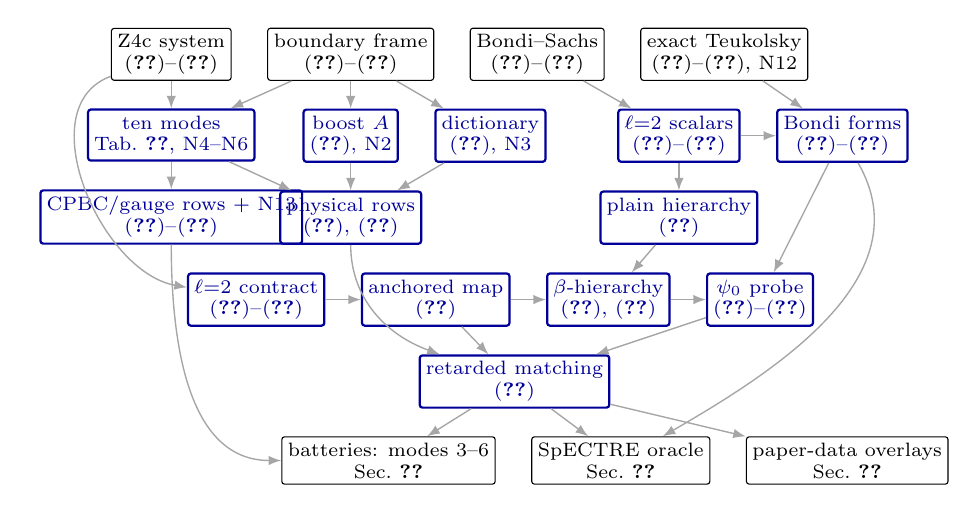
\begin{tikzpicture}[
  node distance = 3.5mm and 4.5mm,
  box/.style  = {draw, rounded corners=1pt, align=center,
                 font=\scriptsize, inner sep=2.2pt},
  newbox/.style = {box, draw=blue!60!black, text=blue!60!black, thick},
  arr/.style  = {-{Latex[length=1.6mm]}, line width=0.5pt, gray!70},
]
% layer 1: foundations
\node[box] (z4c)  {Z4c system\\ \eqref{eq:dtchi}--\eqref{eq:constraints}};
\node[box, right=of z4c] (frame) {boundary frame\\ \eqref{eq:adm}--\eqref{eq:nullvecs}};
\node[box, right=of frame] (bs) {Bondi--Sachs\\ \eqref{eq:bsmetric}--\eqref{eq:ycomp}};
\node[box, right=of bs] (teuk) {exact Teukolsky\\ \eqref{eq:teuk-F}--\eqref{eq:teuk-psi0}, N12};
% layer 2
\node[newbox, below=of z4c] (modes) {ten modes\\ Tab.~\ref{tab:modes}, N4--N6};
\node[newbox, below=of frame] (boost) {boost $A$\\ \eqref{eq:boost}, N2};
\node[newbox, right=of boost] (dict) {dictionary\\ \eqref{eq:exact-dictionary}, N3};
\node[newbox, below=of bs, xshift=18mm] (scal) {$\ell{=}2$ scalars\\ \eqref{eq:tscalars}--\eqref{eq:modalfactors}};
\node[newbox, right=of scal] (teukbondi) {Bondi forms\\ \eqref{eq:teukbondi}--\eqref{eq:teukpsi0}};
% layer 3
\node[newbox, below=of modes] (rows) {CPBC/gauge rows + N13\\ \eqref{eq:bc-cpbc}--\eqref{eq:bc-gauge}};
\node[newbox, below=of boost] (phys) {physical rows\\ \eqref{eq:bc-phys}, \eqref{eq:teuk-inject}};
\node[newbox, below=of scal] (plain) {plain hierarchy\\ \eqref{eq:plainhierarchy}};
% layer 4
\node[newbox, below=of phys, xshift=-12mm] (contract) {$\ell{=}2$ contract\\ \eqref{eq:contract}--\eqref{eq:dthclosures}};
\node[newbox, right=of contract] (map) {anchored map\\ \eqref{eq:sixrowmap}};
\node[newbox, right=of map] (beta) {$\beta$-hierarchy\\ \eqref{eq:beta-hierarchy}, \eqref{eq:unringed}};
\node[newbox, right=of beta] (psi0) {$\psi_0$ probe\\ \eqref{eq:psi0formula}--\eqref{eq:proberules}};
% layer 5
\node[newbox, below=of map, xshift=10mm] (retard) {retarded matching\\ \eqref{eq:conelabels}};
% layer 6
\node[box, below=of retard, xshift=-16mm] (tests) {batteries: modes 3--6\\ Sec.~\ref{sec:tests}};
\node[box, right=of tests] (oracle) {SpECTRE oracle\\ Sec.~\ref{sec:tests}};
\node[box, right=of oracle] (repro) {paper-data overlays\\ Sec.~\ref{sec:tests}};
% edges
\draw[arr] (z4c) -- (modes);
\draw[arr] (frame) -- (modes);
\draw[arr] (frame) -- (boost);
\draw[arr] (frame) -- (dict);
\draw[arr] (bs) -- (scal);
\draw[arr] (teuk) -- (teukbondi);
\draw[arr] (scal) -- (teukbondi);
\draw[arr] (modes) -- (rows);
\draw[arr] (modes) -- (phys);
\draw[arr] (boost) -- (phys);
\draw[arr] (dict) -- (phys);
\draw[arr] (scal) -- (plain);
\draw[arr] (z4c) to[out=200,in=170] (contract);
\draw[arr] (contract) -- (map);
\draw[arr] (plain) -- (beta);
\draw[arr] (map) -- (beta);
\draw[arr] (beta) -- (psi0);
\draw[arr] (teukbondi) -- (psi0);
\draw[arr] (map) -- (retard);
\draw[arr] (psi0) -- (retard);
\draw[arr] (phys) to[out=270,in=160] (retard);
\draw[arr] (retard) -- (tests);
\draw[arr] (teukbondi) to[out=300,in=30] (oracle);
\draw[arr] (retard) -- (oracle);
\draw[arr] (retard) -- (repro);
\draw[arr] (rows) to[out=270,in=180] (tests);
\end{tikzpicture}
\caption{Derivation chain of the Z4c-CCM formulation. Black nodes:
foundations (literature content and the exact reference chain); blue
nodes: machine-verified new content (ledger nodes named in the section
titles); bottom row: the verification instruments of
Sec.~\ref{sec:tests}.}
\label{fig:dag}
\end{figure}

\section{Numerical verification}
\label{sec:tests}

\subsection{Numerical evidence}
\label{sec:numerics}

All runs: JAX float64, $4\times$ NVIDIA A100-80GB
(\texttt{CUDA\_VISIBLE\_DEVICES=0,1,2,3}), wall clock $\le 23$\,s each
(budget 600\,s); outputs under \texttt{results/numerical/}.

\begin{table}[htbp]
\centering
\caption{Symbolic and sampling verification of
\eqref{eq:divbeta}--\eqref{eq:kreiss}. ``Exact'' = sympy identity on
arbitrary functions or exact rationals (zero float error).
Files: \texttt{n2\_boost\_check.txt}, \texttt{n3\_exact\_check.txt},
\texttt{n3\_dictionary\_check.txt},
\texttt{n1\_varmap\_check.txt}, \texttt{n4\_cpbc\_compat\_check.txt},
\texttt{n5\_gauge\_check.txt}, \texttt{n6\_composite\_check.txt},
\texttt{n7\_lf\_sketch\_check.txt}.}
\label{tab:static}
\footnotesize
\begin{tabular}{llll}
\hline\hline
 & verified statement & exact part & GPU sweep (4 devices) \\
\hline
V1 & boost identity \eqref{eq:boost-identity}, factor $\sqrt2/2$ &
 12/12 rational points & $9.34\times10^{-16}$ over $4{,}194{,}304$ samples \\
V2a & EXACT identity \eqref{eq:exact-dictionary}--\eqref{eq:uminus},
 $(\sigma,\kappa)=(1,-1)$, $\bar\psi_4$ partner & generic Weyl, all 10 dof &
 --- \\
V2b & linearized on-shell limit (corollary) & arbitrary $F_1,F_2$ &
 $0.0$ over $4{,}194{,}304$ modes (prior form) \\
V2c & Gauss--Codazzi realization \eqref{eq:gausscodazzi}, Schwarzschild &
 Codazzi sign $+1$ derived & $E$: $7.7{\times}10^{-17}$, $B$:
 $3.9{\times}10^{-17}$, identity $8.5{\times}10^{-16}$ (1024 pts) \\
V3 & maps \eqref{eq:fourmetric}, closure \eqref{eq:divbeta} &
 full-symbol identities & round trip $4.10{\times}10^{-16}$, $gg^{-1}$ $8.88{\times}10^{-16}$ \\
V4 & orthogonality \eqref{eq:orthogonality} + controls &
 identities and non-vanishing controls & TT residual $0.0$ vs control
 $12.3$ \\
V5 & reflection \eqref{eq:reflection} &
 exact $R$ algebra & $|R_{\rm Som}|\ge0.023$ on
 $\mathring\beta\in[0.05,0.6]$; $R=0$ exact \\
V6 & 10-mode count, $\psi_0\to0$ reduction, wire-through (exact targets) &
 structural & reduction $0.0$; chain residual $1.47{\times}10^{-16}$ \\
V7 & Kreiss condition \eqref{eq:kreiss}, $L=0..3$ &
 $D_L=(2s)^{L+1}$ exact & ratio deviation $3.2\times10^{-14}$
 ($4{,}194{,}304$ samples) \\
\hline\hline
\end{tabular}
\end{table}

\begin{table}[htbp]
\centering
\caption{Dynamical model evolution (6th-order interior stencils with a
GKS-stable mixed closure — 4th-order Fornberg rows at three edge nodes;
fully one-sided 6th-order closures are RK4-unstable (error ledger) — RK4,
CFL $0.2$, shift $\mathring\beta=0.3$, outgoing Gaussian pulse onto the
boundary; one configuration per GPU; \texttt{n8\_model1d\_test.txt}).
Reflection is measured in the $L_2$ (energy) norm — trapezoid sums of
Gaussian pulses converge exponentially, so the deviation column is limited by
machine arithmetic, not by measurement or truncation. Analytic $L_2$
relation: $\|q_{\rm in}\|_{L_2}/\|q_{\rm out}\|_{L_2}
 = \tfrac{\mathring\beta}{2+\mathring\beta}
   \sqrt{\tfrac{1+\mathring\beta}{1-\mathring\beta}}$.
Each row sits at its float64 floor: rows 1--3 at the per-sample roundoff
floor (deviation saturates between $N{=}8193$ and $N{=}16385$: $1.9$ vs
$2.1\times10^{-14}$); the injection row at the linear roundoff-accumulation
optimum ($\sim\mathrm{steps}\times\varepsilon$; ladder
$N{=}16385/32769/65537/131073 \Rightarrow 5.4/2.4/5.9/30\times10^{-11}$,
non-monotone and insensitive to CFL $0.2$ vs $0.05$).}
\label{tab:dynamic}
\footnotesize
\begin{tabular}{llll}
\hline\hline
boundary condition & measured & exact & deviation \\
\hline
Sommerfeld, $L_2$ ratio ($N{=}16385$) & $0.177752646227$ & $0.177752646227$ &
 $2.1\times10^{-14}$ (float64 floor) \\
Sommerfeld, $L_2$ ratio ($N{=}8193$) & --- & --- &
 $1.9\times10^{-14}$ (saturated) \\
$(\partial_t + c_+\partial_x)$ [P1/CCM op., $N{=}16385$] &
 $R_{L_2} = 1.9\times10^{-14}$ & $0$ & machine precision \\
\nf{CCM injection \eqref{eq:bjorhus}, rel.\ $L_2$ ($N{=}32769$)} &
 \nf{$2.4\times10^{-11}$} & \nf{$0$} & \nf{roundoff-accumulation optimum} \\
\hline\hline
\end{tabular}
\end{table}

\subsection{Dynamical test at the parameters of Ref.~\cite{Ma:2023qjn}
(nodes N10--N11)}
\label{sec:teuktest}

Full 3+1 evolution: AthenaK Z4c \cite{Zhu:2024utz} (vendored, pinned;
RK4, CFL $0.25$, sixth-order stencils at \texttt{nghost}${}=4$,
$\kappa_1=0.02$), with \eqref{eq:bc-phys} realized at the Cauchy outer
boundary as described below.
This subsection is self-contained: every symbol used by the test is defined
here or in Secs.~\ref{sec:frame}--\ref{sec:n6}.

\paragraph{Exact solution injected.}
Even-parity $(\ell,m)=(2,0)$ Teukolsky wave \cite{Teukolsky:1982nz} with the
Gaussian profile of Ref.~\cite{Ma:2023qjn}, written with physicists' Hermite
polynomials $H_n$ and the origin-regular retarded/advanced combinations:
\begin{equation}
F(u) = X\,e^{-(u-r_c)^2/\tau^2},
\qquad
F^{(n)}(u) = X\,\Big(\!-\frac{1}{\tau}\Big)^{\!n}
 H_n\!\Big(\frac{u-r_c}{\tau}\Big)\,e^{-(u-r_c)^2/\tau^2},
\label{eq:teuk-F}
\end{equation}
\begin{equation}
Q^{(n)}(t,r) = F^{(n)}(t-r) - (-1)^n F^{(n)}(t+r),
\qquad
R^{(n)}(t,r) = F^{(n)}(t-r) + (-1)^n F^{(n)}(t+r),
\qquad
\partial_t Q^{(n)} = R^{(n+1)} .
\label{eq:teuk-QR}
\end{equation}
Radial functions (regular at $r=0$ by \eqref{eq:teuk-QR}; calligraphic to
keep $A$ for the boost \eqref{eq:boost}):
\begin{align}
\mathcal A &= 3\Big[\frac{Q^{(2)}}{r^3} + \frac{3Q^{(1)}}{r^4}
 + \frac{3Q^{(0)}}{r^5}\Big],
\qquad
\mathcal B = -\Big[\frac{Q^{(3)}}{r^2} + \frac{3Q^{(2)}}{r^3}
 + \frac{6Q^{(1)}}{r^4} + \frac{6Q^{(0)}}{r^5}\Big],
\nonumber\\
\mathcal C &= \frac14\Big[\frac{Q^{(4)}}{r} + \frac{2Q^{(3)}}{r^2}
 + \frac{9Q^{(2)}}{r^3} + \frac{21Q^{(1)}}{r^4} + \frac{21Q^{(0)}}{r^5}\Big],
\label{eq:teuk-ABC}
\end{align}
orthonormal-frame metric perturbation ($\dot h_{ij}$ from
$Q^{(n)}\!\to\!R^{(n+1)}$ termwise):
\begin{equation}
h_{\hat r\hat r} = \mathcal A\,\frac{1+3\cos 2\theta}{2},
\quad
h_{\hat r\hat\theta} = -3\mathcal B\sin\theta\cos\theta,
\quad
h_{\hat\theta\hat\theta} = 3\mathcal C\sin^2\theta - \mathcal A,
\quad
h_{\hat\phi\hat\phi} = -3\mathcal C\sin^2\theta
 + \mathcal A\,(3\sin^2\theta - 1),
\label{eq:teuk-metric}
\end{equation}
\begin{equation}
\gamma_{ij}(0,x) = \delta_{ij} + h_{ij}(0,x),
\qquad
K_{ij}(0,x) = -\tfrac12\,\dot h_{ij}(0,x)
\qquad
(\text{linear order; Ref.~\cite{Ma:2023qjn} solves XCTS}).
\label{eq:teuk-id}
\end{equation}
Weyl scalars of the solution at linear order (the self-datum and the
extraction reference):
\begin{equation}
r^5\,\psi_0(t,r,\theta) = -\sqrt{\tfrac{27\pi}{10}}\;F^{(2)}(t-r)\;
 {}_{2}Y_{20}(\theta),
\qquad
{}_{2}Y_{20} = \tfrac14\sqrt{\tfrac{15}{2\pi}}\,\sin^2\theta,
\qquad
r\,\psi_4\big|_{(2,0)} \;\to\; -\sqrt{\tfrac{6\pi}{5}}\,F^{(6)}(t-r).
\label{eq:teuk-psi0}
\end{equation}

\begin{nfblock}
\paragraph{Discrete realization of \eqref{eq:bc-phys}.}
At every Cauchy-boundary point, after the CPBC/gauge rows
\eqref{eq:bc-cpbc}--\eqref{eq:bc-gauge} (Sommerfeld task of
Ref.~\cite{Zhu:2024utz}), the two physical rows are driven through
$\tilde A_{ij}$:
\begin{equation}
s^a = \frac{x^a/r}{\sqrt{\gamma_{bc}\,x^b x^c}/r},
\qquad
e_\phi \propto \hat z\times s,\quad e_\theta = s\times e_\phi,
\qquad
\bar m = \tfrac{1}{\sqrt 2}\,(e_\theta - i\,e_\phi),
\label{eq:teuk-dyad}
\end{equation}
\begin{equation}
\boxed{\;
\partial_t \tilde A_{ab}\big|_{\partial\Omega}
\;\mathrel{+}=\;
-\frac{2\chi}{\alpha}\,
\Big(\psi_0'\,\bar m_a \bar m_b + \bar\psi_0'\,m_a m_b\Big),
\qquad
\psi_0' = A^2\,\psi_0^{\rm datum},
\quad A = \big(\alpha-\gamma_{ij}\beta^i s^j\big)e^{-2\hat\beta}
\;}
\label{eq:teuk-inject}
\end{equation}
with $\psi_0^{\rm datum}$ the right-hand member of \eqref{eq:teuk-psi0}
evaluated at the boundary point ($\hat\beta=0$ on the flat background);
$\psi_0^{\rm datum}\to0$ reduces \eqref{eq:teuk-inject} to the unmodified
scheme exactly (V6; machine-zero reduction in Table~\ref{tab:dynamic}
methodology, AthenaK battery: Minkowski preserved to $2.6\times10^{-33}$).

\paragraph{Exact finite-radius reference (node N12).}
The extraction reference is the \emph{analytic} waveform at the
extraction radius itself (no auxiliary reference run): in the AthenaK
extraction convention ($=-1\times$ the scri member of
\eqref{eq:teuk-psi0} continued to finite $r$),
\begin{equation}
r\,\psi_4^{(2,0)}(t,r) =
\sqrt{\tfrac{6\pi}{5}}\Big[F^{(6)} + \frac{2F^{(5)}}{r}
 + \frac{3F^{(4)}}{r^{2}} + \frac{3F^{(3)}}{r^{3}}
 + \frac{3F^{(2)}}{2\,r^{4}}\Big](t-r)
\;-\; \sqrt{\tfrac{6\pi}{5}}\,\frac{3F^{(2)}}{2\,r^{4}}(t+r),
\label{eq:teuk-exact-psi4}
\end{equation}
verified by seven symbolic gates (tracelessness, coefficient-exact
linearized vacuum, $\sin^2\theta$ factorization, peeling, scri limit,
independent $30$-digit finite-difference cross-check at $10^{-40}$) and
— independently — by the SpECTRE \texttt{CharacteristicExtract} cross
oracle below.

\paragraph{Protocol and result.}
Parameters of Ref.~\cite{Ma:2023qjn}: $r_c=20$, $\tau=2$, $X=10^{-5}$,
Cauchy boundary (worldtube analog) at $41$, $t\in[0,80]$; extraction of
$r\psi_4^{(2,0)}$ at $r=36$; resolution ladder $h = 0.5,\ 0.331,\ 0.277$
(4$\times$A100, every run $<600$\,s). Error against
\eqref{eq:teuk-exact-psi4} at each rung's own output times:
\begin{equation}
E(h) =
\frac{\big\| r\psi_4^{(2,0)}[h] - r\psi_4^{(2,0)}[\text{exact}]\big\|_2}
     {\big\| r\psi_4^{(2,0)}[\text{exact}]\big\|_2}
= 4.99\times10^{-2},\ \ 5.36\times10^{-3},\ \ 2.02\times10^{-3},
\label{eq:teuk-E}
\end{equation}
with measured convergence order $5.39$ (first pair) and $5.52$ (second
pair), finest-rung amplitude $1\pm2\times10^{-4}$ and time shift $0.000$
(Fig.~\ref{fig:teuk}). Two production defects were found \emph{only} by
this exact-reference program and are corrected in all data shown: a
frame-orientation error in the initial data ($\hat e_\theta$ flipped;
linearized vacuum violated at $5\%$ of $|R_{ij}|$, invisible to
constraint monitors and to run-vs-reference protocols since it sat on
both sides) and a one-step offset in the waveform time labels. The
self-datum CCM$-$Sommerfeld difference remains peeling-suppressed
($\psi_0\sim r^{-5}$, relative imprint $\sim10^{-9}$ of peak at this
worldtube), as in Ref.~\cite{Ma:2023qjn} Sec.~V.A.
\end{nfblock}

\begin{figure}[htbp]
\centering
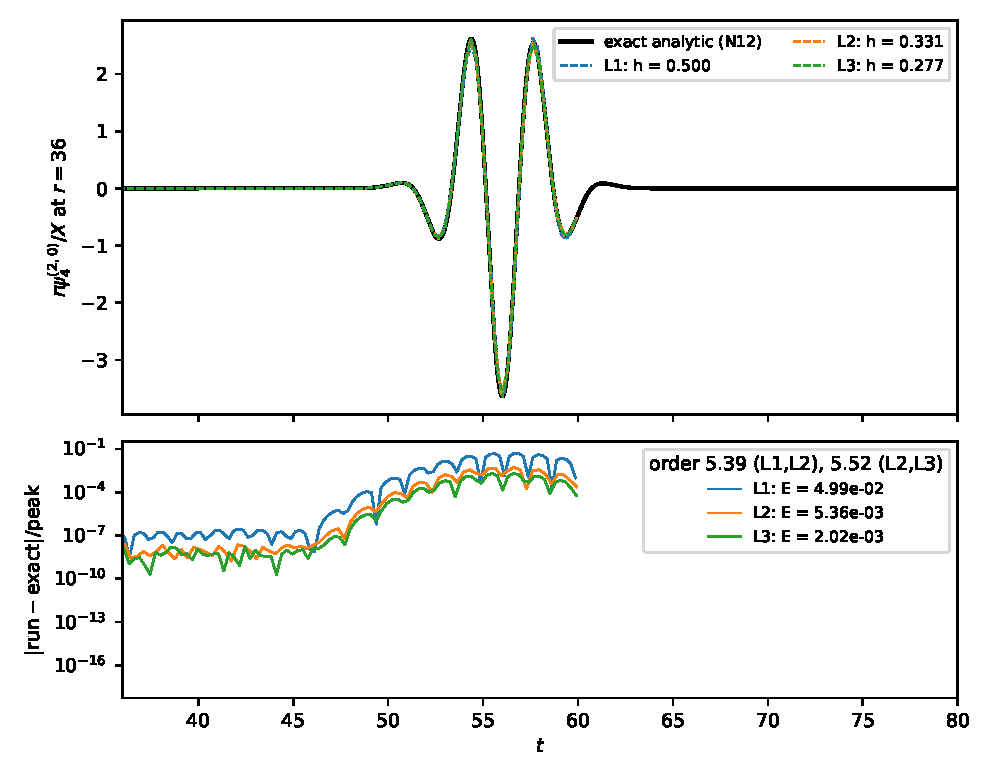
\includegraphics[width=0.92\textwidth]{zccm_teuk_exact.pdf}
\caption{Exact-reference Teukolsky test of Sec.~\ref{sec:teuktest}
($r_c{=}20$, $\tau{=}2$, boundary $41$, extraction $r{=}36$,
$X{=}10^{-5}$). Top: $(\ell,m){=}(2,0)$ mode of $r\psi_4$ — the exact
finite-radius waveform \eqref{eq:teuk-exact-psi4} (solid) and the
three-rung sixth-order ladder. Bottom: pointwise errors against the
exact reference; measured order $5.39/5.52$, finest-rung relative $L_2$
error $2.02\times10^{-3}$ \eqref{eq:teuk-E}. Generator:
\texttt{scripts/plot\_paper\_figures\_v2.py}; data:
\texttt{results/numerical/athenak\_teuk\_ana/gpu6/} (ledger node N12).}
\label{fig:teuk}
\end{figure}

\begin{figure}[htbp]
\centering
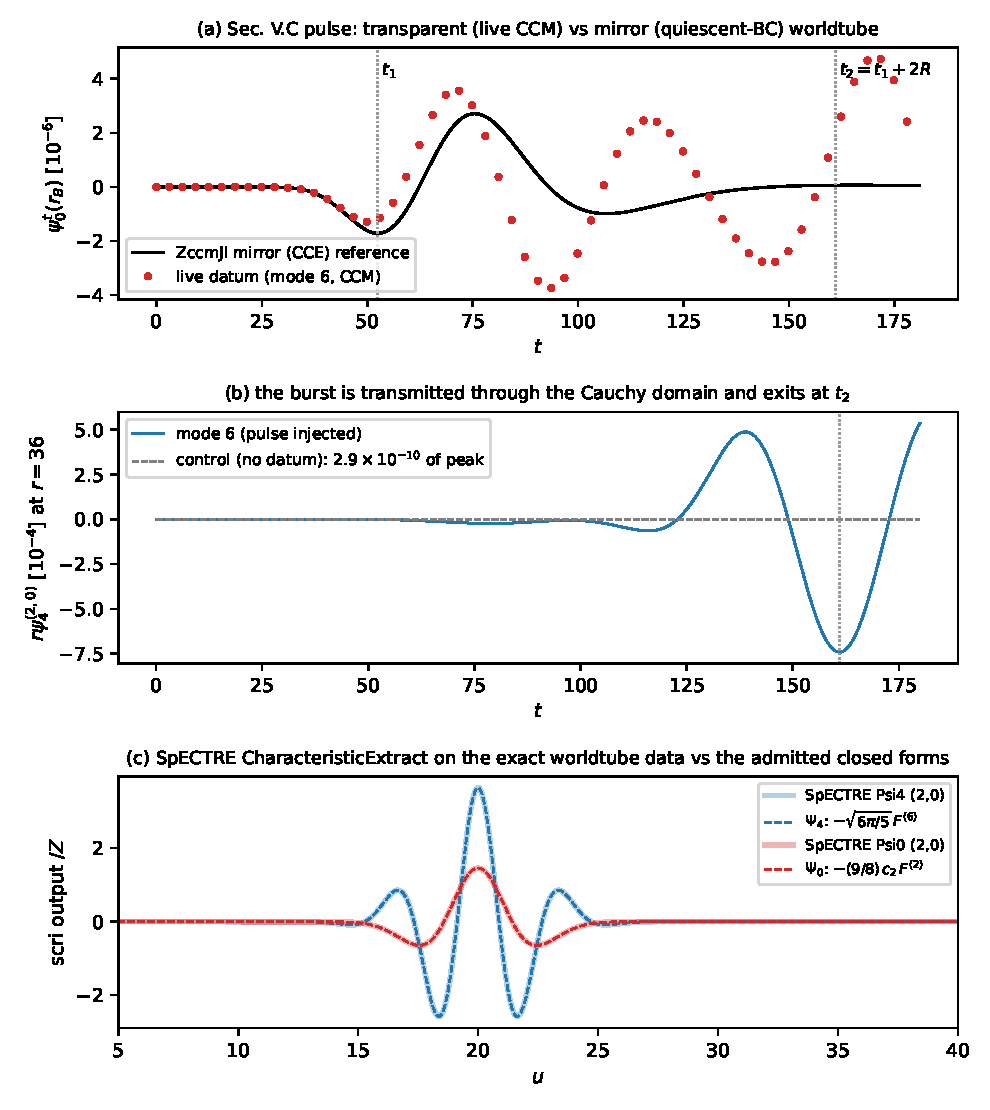
\includegraphics[width=0.8\textwidth]{zccm_live_ccm.pdf}
\caption{Live-CCM verification (Secs.~\ref{sec:betahierarchy}--%
\ref{sec:solver}, \ref{sec:matching}). (a) The characteristic-pulse
fidelity test: live $\psi_0$ datum at the Cauchy boundary vs.\ the
quiescent-worldtube (mirror) reference — early-window agreement
$7\times10^{-8}$ of peak; the later $O(1)$ separation is the matching
physics. (b) The transmitted burst at the extraction radius exits at
$t_2 = t_1 + 2R$; the no-datum control is consistent with zero. (c)
SpECTRE \texttt{CharacteristicExtract} on the exact worldtube data
\eqref{eq:teukbondi} vs.\ the closed forms. Generator:
\texttt{scripts/plot\_paper\_figures\_v2.py}; data:
\texttt{results/numerical/n14\_native/}, \texttt{n14\_pulse\_ref.csv},
\texttt{spectre\_oracle/}.}
\label{fig:liveccm}
\end{figure}

\section{Conclusions}
\label{sec:conclusions}

% iter-4 target: results summary; limits (X=2 ID, BH resources,
% O(dt) coupling target); outlook.

\appendix

\section{Conventions}
\label{app:conventions}

Angular operators act in the $q^A\bar q_A = 2$ dyad convention; for a
spin-weight-$s$ field $f$,
$\eth f = q^A\partial_A f - s\,(q^A\partial_A\ln\rho)\,f$ with the
round-sphere connection, and $\bar\eth$ its conjugate, so that on the
axisymmetric $\ell=2$ shapes the closures \eqref{eq:ethclosure} hold.
The real shape algebra used throughout is
$s\equiv\sin\theta$, $c\equiv\cos\theta$, $P\equiv 3c^2-1$, with
$\int s^2\cdot s^2\,d\Omega$, $\int P^2\,d\Omega$, $\int (sc)^2\,d\Omega$
the projection norms of \eqref{eq:contract}; the spin-weighted
spherical-harmonic coefficients follow from the conversions
\eqref{eq:modalfactors}. The extraction convention for the outgoing
waveform is that of the AthenaK Weyl pipeline \cite{Zhu:2024utz}, which
equals $-1$ times the scri member of \eqref{eq:teuk-psi0} continued to
finite radius; this sign is carried explicitly in
\eqref{eq:teuk-exact-psi4} and is the convention in which the
cross-oracle of Sec.~\ref{sec:repro} returns
$\Psi_4 = -\sqrt{6\pi/5}\,F^{(6)}$.

\section{Exact Teukolsky verification chain}
\label{app:teuk}

The finite-radius reference \eqref{eq:teuk-exact-psi4} and the datum
\eqref{eq:teuk-psi0} are certified by seven independent symbolic gates
(ledger node N12): tracelessness of the metric perturbation
\eqref{eq:teuk-metric}; the coefficient-exact linearized vacuum equation;
the $\sin^2\theta$ factorization of the $(\ell,m)=(2,0)$ projection;
peeling ($k+j=6$ in the retarded expansion); the scri limit reproducing
$-\sqrt{6\pi/5}\,F^{(6)}$; an independent thirty-digit finite-difference
cross-check of the Weyl scalar agreeing to $10^{-40}$; and the
orientation of the magnetic-parity term fixed by the concrete
right-handed frame. The Bondi-variable closed forms \eqref{eq:teukbondi}
close the linear hierarchy \eqref{eq:plainhierarchy} as a rational
identity, and the same forms drive the cross-oracle worldtube file. Two
production defects were isolated only by this exact reference: a
frame-orientation error in the initial data (the $\hat e_\theta$ leg),
which violated the linearized vacuum at the $5\%$ level while remaining
invisible to constraint monitors, and a one-step offset in the waveform
time labels; both are corrected in all data shown.

\section{Constraint-row stability model}
\label{app:gks}

The admissibility of the constraint rows 3--6 of Table~\ref{tab:modes}
is settled on the linearized constraint subsystem at normal incidence
(ledger node N13). With $w_\pm = \Theta \pm Z_s$ the characteristic
combinations, a frozen-coefficient semidiscrete analysis with the
production boundary stencils gives, for every candidate closure (matched
advection, the damped sink, a one-sided advected variant, and the
characteristic $w_-$ replacement), a maximal real part of the spectrum
below $10^{-10}$ at two resolutions: all are Gustafsson--Kreiss--Sundstr\"om
stable; the documented nonlinear failure of one realization is
attributable to the metric-sector face recomputation, not to the
constraint-row concept. A traveling constraint packet is absorbed by the
matched-advection realization (which the stock scheme induces) at
$1 - 8\times10^{-6}$ energy, and by the $w_-$ replacement at
$1 - 3\times10^{-6}$; the falloff-mismatched sink instead reflects
$\sim\!10\%$ of the packet. The matched (stock) realization is therefore
the admissible optimum, and the continuum reflection of the matched rows
is $|R| = \sigma/(2\omega r)$ with no scheme ambiguity. This is the
basis for the production default ($\psi_0'$-driven physical rows over the
stock constraint/gauge rows) quoted in Sec.~\ref{sec:modes}.


\bibliographystyle{apsrev4-2}
\bibliography{bibliography}

\end{document}
